\begin{itemize}
  \item Extrapolation error: unseen state-action pairs are estimated to have unrealistic values
  \item Error can be attributed to mismatch in distribution of data induced by policy and data contained in the batch
  \item BCQ uses state-conditioned generative model to produce only previously seen actions
  \item Extrapolation error can be attributed to several causes:
  \begin{itemize}
    \item Absent data: $(s,a)$ is unavailable
    \item Model bias
    \item Training mismatch
  \end{itemize}
  \item Off-policy algorithms (e.g. DDPG) deteriorate in perfomance when data is uncorrelated and value estimate produced by the Q-net diverges
  \item Off-policy algorithms are ineffective when learning \textit{truly off-policy}
  \item Three different batch tasks: final buffer, concurrent, and imitation
  \item Behavioral agent consistently outperformed the off-policy agent trained with DDPG
  \item Batch-constrained policies trained to select actions with respect to three objectives:
  \begin{itemize}
    \item Minimize distance of selected actions to data in the batch
    \item Lead to states where familiar data can be observed
    \item Maximize the value function
  \end{itemize}
  \item BCQ generates plausible candidate actions with high similarity to the batch and selects the highest valued action using a learned Q-network
  \item Actions outputted using a generative model $G_{w}(s)$
  \item A perturbation model $\xi_{\phi}(s,a,\Phi)$ which is used to increase the diversity of the actions
  \item The choice of the number of actions to sample $n$ and $\Phi$ creates a trade-off between imitation learning and RL
  \item Also uses a modified Clipped Double Q-Learning to estimate value by taking a convex combination of two Q-networks
  \begin{figure}[h]
    \centering
    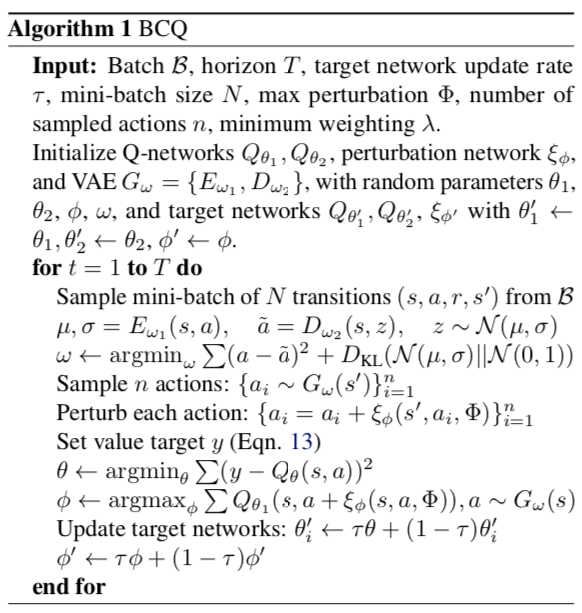
\includegraphics[width=0.5\textwidth]{../../imgs/bcq.png}
  \end{figure}

  \item Experiments and results
  \begin{itemize}
    \item MuJoCo environments in OpenAI gym
    \item Baselines: DDPG, DQN, BC, and VAE-BC
    \item Tasks: HalfCheetah, Hopper, Walker2d
    \item BCQ is the only one that succeeds at all tasks, matching or outperforming BC
    \item Achieves high performance in very few iterations, able to disentangle poor and expert actions
    \item Suggests that extrapolation error has been successfully mitigated, BCQ is able to accurately estimate the true Q-value
  \end{itemize}

\end{itemize}